\documentclass{article}

\usepackage[preprint]{neurips_2025}

\usepackage[utf8]{inputenc}
\usepackage[T1]{fontenc}
\usepackage{hyperref}
\usepackage{url}
\usepackage{booktabs}
\usepackage{amsfonts}
\usepackage{nicefrac}
\usepackage{xcolor}
\usepackage{graphicx}
\usepackage{amsmath}
\usepackage{amssymb}
\usepackage{listings}
\usepackage{menukeys}
\usepackage{hwemoji}

% LaTeX code style with line numbers
\lstdefinestyle{latexstyle}{
    language=[LaTeX]TeX,
    backgroundcolor=\color{white},
    basicstyle=\ttfamily\small,
    keywordstyle=\color{blue},
    commentstyle=\color{gray},
    stringstyle=\color{red!70!black},
    numbers=left,
    numberstyle=\tiny\color{gray},
    numbersep=6pt,
    frame=single,
    rulecolor=\color{black!20},
    breaklines=true,
    showstringspaces=false
}

\lstset{style=latexstyle}
\usepackage{caption}
\usepackage{subcaption}
\usepackage{tikz}
\usetikzlibrary{trees}

% Define remark environment
\newenvironment{remark}{\begin{quote}\textbf{Remark:}}{\end{quote}}

\title{\LaTeX{} Compilation: Challenges in the Era of LLMs}

\author{%
  Tianyou Liu$^\dag$ \\
  Southern University of Science and Technology \\
  \texttt{12511307@mail.sustech.edu.cn} \\
  \And
  Ziqiang Li$^\dag$ \\
  Alibaba \\
  \texttt{liziqiang.lzq@alibaba-inc.com} \\
  \And
  Yansong Li \\
  Liii Network \\
  \texttt{yansong@liii.pro} \\
  \And
  Xurui Liu \\
  Tsinghua University \\
  \texttt{liuxr21@mails.tsinghua.edu.cn} \\
}

\newcommand{\dagfootnote}{{\let\thefootnote\relax\footnotetext{$^\dag$These authors contributed equally to this work.}}}

\begin{document}

\maketitle

\dagfootnote

\begin{abstract}
As large language models (LLMs) increasingly assist scientific writing, limitations and significant token cost of the TeX become more and more visible. This paper analyzes TeX's fundamental defects in compilation and user experience design to illustrate its limitations on compilation efficiency, generated semantics, error localization, and tool ecosystem in the era of LLMs. As an alternative, \textbf{Mogan STEM}, a WYSIWYG structured editor is introduced. Mogan outperforms TeX in the above aspects by its efficient data structure, fast rendering, and on-demand plugin loading. Extensive experiments are conducted to verify the benefits on compilation/rendering time, performance in LLM tasks. What's more, we show that due to Mogan's lower information entropy, it is more efficient to use \texttt{.tmu} (document format of Mogan) to fine-tune LLMs than TeX. Therefore, we launch an appeal for larger experiments on LLM training using the \texttt{.tmu} format.
\end{abstract}


\section{A Brief History of \TeX}

Numerous derivatives of TeX have been emerged in past decades, with LaTeX being the most prominent. Built as a macro language on top of TeX, LaTeX significantly simplifies its usage, allowing users to leverage TeX's powerful typesetting capabilities without needing a deep understanding of intricate commands. By defining commands and templates that align with standard typesetting practices, LaTeX has made the production of scientific literature and books far more efficient and accessible, eventually becoming the de facto standard for scientific document preparation.

In the academic field, the TeX system and LaTeX in particular have become the standard of the scientific community thanks to its exceptional mathematical typesetting capabilities. The core design of TeX originates from the pioneering work of Donald Knuth \citep{knuth1984texbook}. The American Mathematical Society (AMS) strongly encourages mathematicians to submit manuscripts using TeX, and widespread adoption by world-class publishers such as Wesley and IEEE has made it a staple for books and journals. Consequently, TeX occupies a pivotal position in the production of academic papers and monographs, serving as a vital tool for scholarly communication and knowledge dissemination.

However, TeX's original design and its subsequent development trajectory have resulted in numerous legacy issues. This article primarily examines the underlying architecture of TeX and explains why certain design choices have led to significant problems.

On another note, it was long believed that ``What You See Is What You Get'' (WYSIWYG) was incompatible with structured editing. The emergence of TeXmacs, however, proved this assumption fundamentally incorrect. Professor Joris from \'Ecole Polytechnique wrote a critique on this subject (see Joris et al.~\citep{van_der_hoeven_gnu_2001, liiistem2025}). The design philosophy of LaTeX has inspired a series of similar editing software; beyond the aforementioned TeXmacs, these include LyX and the recently popular Typst.

Notably, the formula rendering in Typst and TeXmacs is completely independent of the TeX system, whereas LyX serves as a front-end for TeX. While this article contains significant criticism of the TeX system, we wish to clarify our stance: we are by no means denying TeX's historical status, nor do we suggest it was outdated for its time. We simply argue that today---especially in an era of rapidly advancing AI tools---TeX's underlying design presents many issues.


\section{An Introduction to \TeX{} Compilation Principles}

\begin{example}[Minimal example of LaTeX code]
\label{ex:minimal}
\begin{verbatim}
\documentclass{article}
\usepackage{siunitx}
\begin{document}
Hello, World! from \LaTeX.
The speed of light is \SI{299792458}{\meter\per\second}.
\end{document}
\end{verbatim}
\end{example}

Example~\ref{ex:minimal} shows a minimal example of LaTeX code. The source code comprises two parts: the preamble, which includes the \verb|\documentclass| and \verb|\usepackage| commands, and the document body, which is enclosed within the \verb|\begin{document}| and \verb|\end{document}| environment. The preamble serves as the configuration section for the document, where global settings such as page layout, fonts, and macro definitions are specified. The \verb|\documentclass| command is used to select a document template (class) that controls the overall structure and formatting. The \verb|\usepackage| command imports packages that provide additional functionality, such as mathematical symbols, special characters, or custom formatting options.

\begin{table}[htbp]
\centering
\caption{\LaTeX{} file extensions and their descriptions}
\label{tab:latex-ext}
\begin{tabular}{ll}
\toprule
\textbf{Extension} & \textbf{Description} \\
\midrule
\texttt{.tex} & Source file containing document content \\
\texttt{.sty} & Style file (package) \\
\texttt{.cls} & Class file defining document structure \\
\texttt{.bst} & BibTeX bibliography style file \\
\bottomrule
\end{tabular}
\end{table}

Table~\ref{tab:latex-ext} lists the main file extensions used in the LaTeX ecosystem. The source code is written in plain text using a text editor and saved with a \texttt{.tex} extension. The LaTeX engine then processes this source file to generate the final output. The engine reads the source file sequentially, expanding macros and processing commands to produce a document in the desired output format (typically DVI or PDF).

\begin{table}[htbp]
\centering
\caption{\LaTeX{} auxiliary file extensions, tools, and descriptions}
\label{tab:latex-aux}
\begin{tabular}{lll}
\toprule
\textbf{Extension} & \textbf{Tool} & \textbf{Description} \\
\midrule
\texttt{.aux} & \texttt{latex}/\texttt{pdflatex} & Auxiliary file for cross-references \\
\texttt{.log} & \texttt{latex}/\texttt{pdflatex} & Log file containing compilation messages \\
\texttt{.toc} & \texttt{latex}/\texttt{pdflatex} & Table of contents file \\
\texttt{.bbl} & \texttt{bibtex} & Bibliography file \\
\texttt{.blg} & \texttt{bibtex} & Bibliography log file \\
\bottomrule
\end{tabular}
\end{table}

Table~\ref{tab:latex-aux} shows the auxiliary files generated during compilation. The compilation process typically involves multiple passes: the first pass generates auxiliary files, and subsequent passes use these files to resolve cross-references, citations, and other dynamic elements. This multi-pass approach is necessary because LaTeX is a batch-processing system that does not maintain state between runs \citep{lamport1994document}.


\section{Fundamental Defects in \TeX{}'s Compilation Design}
\label{sec:fundamental}

\subsection{Batch Model Limitations: Unidirectionality, Weak Semantics, and Delayed Feedback}

\subsubsection{Unidirectional and One-off Processing Flow}

The core workflow of TeX is inherently unidirectional and batch-oriented. It sequentially reads the source file from beginning to end, expanding macros and processing commands in a single pass. This design, while simple and efficient for its original purpose, creates significant limitations for modern document editing workflows.

The unidirectional nature means that once the compiler has processed a section of the document, it cannot go back to modify it based on information that appears later. This is particularly problematic for cross-references, where the target may appear after the reference itself. The typical workaround is to use multiple compilation passes, but this introduces significant overhead and complexity.

\subsubsection{Tight Coupling Between Compilation and Semantic Phases}

In TeX, the lexical analysis, parsing, and semantic analysis phases are tightly coupled. The macro expansion mechanism, which is central to TeX's operation, operates at the character level without clear separation between these phases. This design choice has several consequences:

\begin{itemize}
    \item \textbf{Fragile Parsing:} The parser must handle expanded macros, making it difficult to provide meaningful error messages.
    \item \textbf{Limited Optimization:} Without clear phase separation, optimizations that could be applied at specific stages are difficult to implement.
    \item \textbf{Debugging Difficulties:} Errors may manifest far from their actual source due to macro expansion.
\end{itemize}

\subsubsection{Lagged Manifestation and Ambiguous Localization of Errors}

TeX's error reporting is notorious for being cryptic and unhelpful. When an error occurs, the compiler often reports it at a location far removed from the actual source of the problem. This is due to several factors:

\begin{enumerate}
    \item Macro expansion can propagate errors across large portions of the document.
    \item The batch processing model means that errors accumulate before being reported.
    \item Error messages are often technical and do not provide actionable guidance.
\end{enumerate}

For example, a missing brace several pages earlier might cause an error message that appears to indicate a problem in a completely different location. This makes debugging LaTeX documents a time-consuming and frustrating experience, especially for users who are not deeply familiar with the system.

\subsection{Compatibility Dilemma Beneath a Unified Syntax}

LaTeX's success has created a massive ecosystem of packages and classes, each extending the language in various ways. However, this extension mechanism relies on macro redefinition, which is inherently fragile. When two packages attempt to redefine the same command, conflicts can arise that are difficult to diagnose and resolve.

\begin{table}[htbp]
\centering
\caption{Common \LaTeX{} Hook Directives and Descriptions}
\label{tab:latex-hooks}
\begin{tabular}{lp{10cm}}
\toprule
\textbf{Hook} & \textbf{Description} \\
\midrule
\texttt{\textbackslash AtBeginDocument} & Executed at the beginning of the document body \\
\texttt{\textbackslash AtEndDocument} & Executed at the end of the document \\
\texttt{\textbackslash AtBeginDvi} & Executed when the first page is shipped out \\
\bottomrule
\end{tabular}
\end{table}

Table~\ref{tab:latex-hooks} shows some common hook directives. While hooks provide a mechanism for packages to coordinate their initialization, they cannot fully resolve the fundamental tension between extensibility and compatibility. The order of package loading becomes critical, and users must often engage in trial-and-error to find a working configuration.

\subsection{Alienation of the Tool Ecosystem}

\subsubsection{Multi-pass Compilation: A Fragile Stopgap}

In LaTeX, the accurate generation of cross-references, tables of contents, and bibliographies relies on multiple compilation passes to make up for the absence of internal state. The typical workflow involves a first pass that generates auxiliary files (like \texttt{.aux} and \texttt{.toc}) to record state, followed by subsequent passes that read these files to populate cross-references, page numbers, or chapter titles.

If the document includes citations, external tools such as BibTeX or Biber must also be integrated into the process. For example, the standard procedure for a document with references often follows the sequence: \texttt{pdflatex} $\rightarrow$ \texttt{bibtex} $\rightarrow$ \texttt{pdflatex} $\rightarrow$ \texttt{pdflatex}.

This mechanism imposes several burdens:

\begin{itemize}
    \item \textbf{State Fragmentation:} Document state is scattered across multiple external files.
    \item \textbf{Cognitive Load:} Users must master complex ``compilation rituals.'' For instance, failure to run BibTeX results in all citation numbers appearing as \texttt{??}.
    \item \textbf{Debugging Difficulties:} Error tracing is notoriously difficult because errors in auxiliary files (e.g., corrupted \texttt{.aux} files) are hard to diagnose.
\end{itemize}

\subsubsection{Long-Term Suppression of the Tool Ecosystem}

The complexity of the LaTeX compilation pipeline has suppressed innovation in the tool ecosystem. Building tools that interact with LaTeX requires understanding the intricate details of the compilation process, the various auxiliary files, and the interactions between different packages. This high barrier to entry has limited the development of sophisticated tools for LaTeX document analysis, refactoring, and collaboration.

\subsection{Comparison: Design Paradigms of Structured and Incremental Systems}

In contrast to TeX's batch-oriented design, modern structured editors like Mogan STEM adopt an incremental approach. Documents are represented as structured trees rather than flat text, and changes are propagated immediately through the document structure. This enables:

\begin{itemize}
    \item \textbf{Immediate Feedback:} Changes are visible instantly without waiting for compilation.
    \item \textbf{Precise Error Localization:} Errors are associated with specific nodes in the document tree.
    \item \textbf{Semantic Understanding:} The editor maintains a rich representation of the document structure.
\end{itemize}


\section{Limitations of \TeX{} in User Experience Design}
\label{sec:ux}

\TeX{} and its derivative, the \LaTeX{} ecosystem, have long occupied a central position in the field of academic typesetting. However, the overall user experience has failed to evolve in sync with the advancement of computing environments and user expectations. From the continuous bloating of distribution sizes to the performance and interaction barriers imposed by the compilation model, and further to the long-standing engineering defects in language design, the \TeX{} ecosystem falls short in modern writing contexts---particularly regarding "usability," "maintainability," and "adaptability to modern workflows." This section analyzes the limitations of \TeX{}'s user experience design from multiple dimensions, including deployment costs, language structure, and practical user experience.

\subsection{Issues with Distribution Scale and Deployment Models}

\begin{figure}[htbp]
\centering
\includegraphics[width=0.8\textwidth]{figure/iso_size.pdf}
\caption{TeX Live ISO Size Trends}
\label{fig:texlive-size}
\end{figure}

Figure~\ref{fig:texlive-size} illustrates the trend in file size for the most popular TeX Live ISO from 2008 to 2025. The horizontal axis represents the year, and the vertical axis represents file size in GB. Starting at 2.4~GB in 2008, the line shows an overall upward trajectory, reaching 5.9~GB by 2025. Despite minor fluctuations (such as a drop to 1.9~GB in 2010 and a slight dip to 3.2~GB in 2018), the long-term trend demonstrates a nearly twofold increase in size, reflecting the continuous expansion of software packages.

This volumetric growth is primarily driven by TeX Live's role as a comprehensive \LaTeX{} distribution, which constantly integrates new fonts, documentation, multi-language support, and packages to adapt to user needs and technological advancements. For instance, while early versions focused on core functionality, later iterations incorporated extensive PDF support, graphics libraries, and extensions, resulting in volume bloat.

However, this continuous expansion warrants critical reflection. Taking TeX Live as an example, a significant portion of its distribution volume consists of documentation sets and font resources. For beginners or light users requiring only basic typesetting functions, such overhead constitutes a clear redundant burden, consuming installation time, disk space, and maintenance effort. Although the \TeX{} ecosystem emphasizes modularity at the package level, the distribution strategy (as illustrated in Figure~\ref{fig:texlive-installer}) still prioritizes full installation as the default. Minimalist installation options, while available, are neither highlighted nor widely adopted. Consequently, most users default to the full version, effectively "normalizing" the issues of bloat and resource waste.

While distributions like MikTeX attempt to address this, a more aggressive promotion of lean versions in default configurations by making documentation, examples, and large font sets optional is far more rational in terms of efficiency, resource utilization, and environmental impact, particularly in network- or storage-constrained scenarios.

\begin{figure}[htbp]
\centering
\includegraphics[width=0.8\textwidth]{figure/texlive-installer.png}
\caption{TeX Live Installer}
\label{fig:texlive-installer}
\end{figure}

Figure~\ref{fig:texlive-installer} illustrates the complex installation interface. In contrast, Mogan STEM uses an on-demand plugin loading mechanism, where features are only loaded when needed. This significantly reduces the installation size and startup time.

\subsection{Real-World Performance Dilemma}

The performance of \LaTeX{} compilation degrades significantly with document complexity. Documents with extensive cross-references, bibliographies, or complex mathematical content require multiple passes and can take minutes to compile. This creates a frustrating edit-compile-view cycle that interrupts the writing flow.

\subsection{Intrinsic Weakness: Absence of Engineering Standards}

\LaTeX{} lacks formal engineering standards for package development. While the \texttt{lppl} license provides some guidance, there are no enforced standards for:

\begin{itemize}
    \item Package documentation quality
    \item API stability and versioning
    \item Error handling and reporting
    \item Testing and validation
\end{itemize}

This has led to a fragmented ecosystem where package quality varies widely, and compatibility issues are common \cite{interview2021}.

\begin{table}[htbp]
\centering
\caption{Core Structural Contradictions in \LaTeX2e\ Language Design and their Engineering Consequences}
\label{tab:latex-contradictions}
\begin{tabular}{p{3.5cm}p{5cm}p{4cm}}
\toprule
\textbf{Contradiction} & \textbf{Description} & \textbf{Impact} \\
\midrule
Global Naming vs.\ Modularity & \LaTeX2e\ lacks namespaces; all commands and variables share a global symbol table & High risk of package conflicts; loading order directly affects behavior; system fragility \\
Text Substitution vs.\ Structured Interfaces & Macros are essentially untyped token substitutions, lacking parameter signatures and type systems & Static checking is difficult; function interfaces are uncomposable; parameter passing is error-prone \\
Local State via Grouping vs.\ Compiler Awareness & State management relies on TeX's grouping and rollback mechanism rather than explicit variable scoping & Compilers cannot resolve scope; state leakage and logical errors are difficult to detect \\
Conventional Interfaces vs.\ Automatic Verification & Interface constraints rely on documentation and voluntary compliance, not language-level enforcement & Parameter types/counts cannot be statically verified; errors are only exposed at runtime \\
Compatibility vs.\ Modern Features & To maintain compatibility with \LaTeX2e, implementation of new features is cumbersome & Requires reliance on advanced packages like \texttt{xparse} or complex hacks; high learning and maintenance costs \\
\bottomrule
\end{tabular}
\end{table}

\subsection{User Experience Barriers from a Practical Perspective}

For users, the \LaTeX{} experience is characterized by:

\begin{enumerate}
    \item \textbf{Steep Learning Curve:} Understanding macro expansion, package interactions, and compilation workflows requires significant investment.
    \item \textbf{Cryptic Error Messages:} Error messages often require deep knowledge of \TeX{} internals to interpret.
    \item \textbf{Fragile Workflows:} Small changes can break the compilation in unexpected ways.
    \item \textbf{Limited Tooling:} Compared to modern IDEs, \LaTeX{} editors offer limited refactoring, navigation, and debugging capabilities.
\end{enumerate}

\subsection{Contributions and Constraints of \LaTeX3}

\LaTeX3 represents an effort to modernize the \LaTeX{} codebase by introducing a more structured programming layer (\texttt{expl3}). While these improvements address some of the technical debt accumulated over decades, they remain constrained by the need for backward compatibility. The improvements are incremental rather than fundamental, and users must still engage with the legacy macro system for many tasks.

\subsection{Limitations of Modern Collaboration Platforms: A Case Study of Overleaf}

In response to \LaTeX{}'s structural deficiencies regarding collaboration support and usability, the academic community has advanced a series of improvement measures. Among these, online collaboration platforms, exemplified by Overleaf, have significantly streamlined the user experience and reduced the technical barrier to entry \cite{overleaf_docs}.

\subsubsection{Key Improvements by Overleaf}

Overleaf has addressed some of \LaTeX{}'s usability issues by providing:

\begin{itemize}
    \item Real-time collaboration features
    \item Simplified compilation management
    \item Version control integration
    \item Template libraries for common document types
\end{itemize}

\subsubsection{Constraints of Underlying Architecture}

However, Overleaf cannot overcome the fundamental limitations of \LaTeX{}'s architecture:

\begin{itemize}
    \item Compilation is still batch-oriented and slow
    \item Error messages remain cryptic
    \item Real-time preview requires frequent recompilation
    \item Collaboration is at the text level, not the semantic level
\end{itemize}

\subsubsection{Impact on Trajectory of Technological Evolution}

By providing a veneer of usability over \LaTeX{}'s fundamental limitations, platforms like Overleaf may have inadvertently slowed the adoption of genuinely superior alternatives. Users who might otherwise seek better solutions are satisfied with incremental improvements to the existing system.


\section{Mogan STEM: A WYSIWYG Structured Editor}
\label{sec:mogan}

Since last year, the maintainers of the Chinese TeXmacs community have developed Mogan STEM~\cite{moganstem2025} and a commercial version, Liii STEM~\cite{liiistem2025}, based on GNU TeXmacs. Currently, Mogan STEM and TeXmacs stand as the world's only WYSIWYG structured editors. Table~\ref{tab:mogan-vs-other} compares Mogan STEM with several other editors currently available on the market.

\begin{table}[htbp]
\centering
\caption{Comparison between Mogan STEM and alternative editors}
\label{tab:mogan-vs-other}
\begin{tabular}{lcccc}
\toprule
\textbf{Editor} & \textbf{WYSIWYG} & \textbf{Structured} & \textbf{Unicode Support} & \textbf{\TeX{} Compatibility} \\
\midrule
\textbf{Mogan STEM} & Yes & Yes & Yes & Partial \\
\textbf{TeXmacs} & Yes & Yes & Partial & Partial \\
\textbf{TeX/LaTeX} & No & Yes & Partial & Full \\
\textbf{Word} & Yes & No & Partial & Incompatible \\
\textbf{LyX} & Partial & Yes & Partial & Full \\
\textbf{Typst} & No & Yes & Yes & Partial \\
\bottomrule
\end{tabular}
\end{table}

The core technical challenge in achieving the WYSIWYG capability of Mogan STEM lies in the representation and rendering of mathematical formulas. Unlike \TeX{}, which represents formulas through layout-oriented markup in the form of typesetting instructions, Mogan STEM adopts a tree-based, functional representation for both mathematical formulas and the document structure itself. The following discussion evaluates this mechanism with specific examples.

\subsection{Tree-Structured Formulas and Document Structure}
\label{sec:tree-struc-on-mogan}

Unlike \LaTeX{}'s compilation model, which centers on linear text and macro expansion, TeXmacs features an explicit tree-based document structure designed from the outset. Document components---such as chapters, formulas, citations, and typesetting elements---exist as structured nodes, rather than being implicitly embedded within macro calls or token streams. This architectural distinction directly impacts citation updates, compilation efficiency, and the interactive user experience.

A fraction serves as a primary example of this difference. In \TeX{}, a fraction is represented as \verb|\frac{1}{2}|; internally, the compiler processes \verb|\frac|, \verb|{1}|, and \verb|{2}| serially. In Mogan STEM, however, the fraction is represented at the underlying layer as the Scheme code \verb|(frac "1" "2")|.\footnote{Note that Mogan STEM is \textbf{WYSIWYG}; therefore, when inputting $\frac{1}{2}$, the user does not type \texttt{(frac 1 2)}, but instead presses \keys{Alt + F} to input it visually!} This forms a tree structure, as illustrated in Figure~\ref{fig:frac-tree}.

\begin{figure}[htbp]
\centering
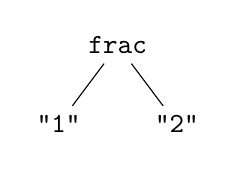
\begin{tikzpicture}[
    level 1/.style={sibling distance=15mm, level distance=10mm},
    every node/.style={align=center}
]
\node {\texttt{frac}}
    child {node {\texttt{"1"}}}
    child {node {\texttt{"2"}}};
\end{tikzpicture}
\caption{The Tree Structure of Mogan Formulas}
\label{fig:frac-tree}
\end{figure}

Let us consider another example:

\begin{equation}
\label{eq:tree-struc}
\int_{a}^{b} f(x) \mathrm{d}x = \left[ F(x) \right] \big|_{a}^{b}
\end{equation}

Its Scheme representation is as follows:
\begin{lstlisting}[caption={Scheme representation of integral expression},label={lst:scheme-integral},upquote=true]
> `(math (concat (big "int") (rsub "a") (rsup "b") "f" (around* "(" "x" ")") "<mathd>x=" (around* "<nobracket>" (around* "[" (concat "F" (around* "(" "x" ")")) "]") "|") (rsub "a") (rsup "b")))
\end{lstlisting}

Note that the segment $\left[ F(x) \right] |$ is managed via the tree structure illustrated in Figure~\ref{fig:tree-representation}. Consequently, even if a user omits a parenthesis or two, this omission does not negatively affect the rendering of the entire mathematical expression in Mogan.

\begin{figure}[htbp]
    \centering
    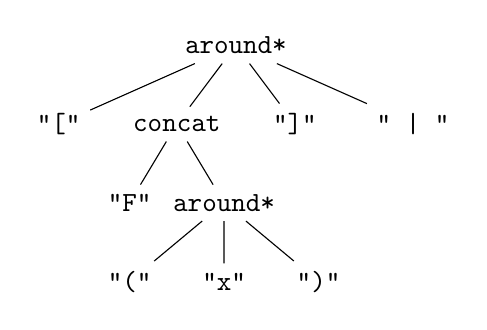
\begin{tikzpicture}[
        level 1/.style={sibling distance=15mm, level distance=10mm},
        level 2/.style={sibling distance=12mm, level distance=10mm},
        level 3/.style={sibling distance=12mm, level distance=10mm},
        every node/.style={align=center}
    ]
    \node {\texttt{around*}}
        child {node {\texttt{"["}}}
        child {node {\texttt{concat}}
            child {node {\texttt{"F"}}}
            child {node {\texttt{around*}}
                child {node {\texttt{"("}}}
                child {node {\texttt{"x"}}}
                child {node {\texttt{")"}}}
            }
        }
        child {node {\texttt{"]"}}}
        child {node {\texttt{" | "}}};
    \end{tikzpicture}
    \caption{Tree representation of $ [F (x)] |$}
    \label{fig:tree-representation}
\end{figure}

Unlike \TeX{}, this tree structure exists at the rendering level, not the syntax level. In fact, many long-time users of Mogan and TeXmacs cannot write a single line of Scheme code! This rendering-level tree structure offers two distinct advantages:

\begin{enumerate}
    \item \textbf{Local Scoping of Input Errors:}
    \begin{itemize}
        \item Errors do not cause the entire document to fail rendering (a major drawback of \LaTeX{}).
        \item Local edits do not trigger global layout instability (a major drawback of MS Word).
    \end{itemize}

    \item \textbf{Parallel Processing:} The CPU renders data in parallel rather than serially, which significantly accelerates rendering speed.
\end{enumerate}

Let's look at another example. For a two-line layout like Figure~\ref{fig:double-line}, the representation is:
\begin{lstlisting}
(document "Mogan Logo" "(figure )" (itemize (document (concat (item) "WYSIWYG Writing") "")))
\end{lstlisting}

\begin{figure}[htbp]
\centering
\includegraphics[width=0.3\textwidth]{figure/double-line.png}
\caption{Image insertion between lines}
\label{fig:double-line}
\end{figure}

\begin{figure}[htbp]
\centering
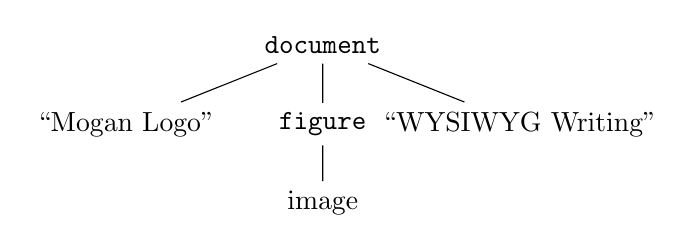
\begin{tikzpicture}[
    level 1/.style={sibling distance=25mm, level distance=10mm},
    level 2/.style={sibling distance=25mm, level distance=10mm},
    every node/.style={align=center}
]
\node {\texttt{document}}
    child {node {``Mogan Logo''}}
    child {node {\texttt{figure}}
        child {node {image}}
    }
    child {node {``WYSIWYG Writing''}};
\end{tikzpicture}
\caption{Mogan's multi-line data structure}
\label{fig:multiline-mogan}
\end{figure}

This corresponds to the tree structure shown in Figure~\ref{fig:multiline-mogan}. As the figure demonstrates, in Mogan, each line of content and every image block maps to an independent leaf node within the tree. Consequently, modifying an image (e.g., resizing or replacing it) triggers a re-render of only that specific leaf node, without disrupting the layout of surrounding lines. This design effectively resolves the issue common in unstructured editors such as Word, where local modifications often lead to global layout chaos.

\subsection{Functional Symbol Representation}

In \TeX{}, all mathematical symbols and fonts are represented as strings. However, in Mogan STEM, certain special symbols are defined via functions. For instance, the inner product $\langle \cdot \rangle$, as shown in Equation~\ref{eq:braket}, is an anonymous function that automatically scales according to the symbols it contains. While this is similar to \verb|\langle \rangle| in \LaTeX{}, the difference lies in the fact that, as a complete function, the left and right brackets always renders a unified pair rather than isolated characters. To obtain a single bracket, the user manually deletes the undesired character from the rendered pair.

\begin{equation}
\label{eq:braket}
\left\langle \int \right\rangle \langle f \rangle
\end{equation}

This functional approach contrasts with \LaTeX{}'s macro-based approach, where \verb|\frac{a}{b}| relies on positional arguments and implicit grouping.

\subsection{Fast Reference Rendering}

Taking bibliographic citations as an instance: in the \LaTeX{} ecosystem, \verb|\cite| serves merely as a macro interface, with actual citation relationships established indirectly via intermediate files such as \verb|.aux| and \verb|.bbl|. Consequently, any modification to bibliography entries typically necessitates multiple global compilation cycles, exemplifying a classic batch processing model. In contrast, Mogan STEM treats citation relationships as structural links directly embedded in the document tree. To update a reference, the system performs only a local search and re-renders the specific leaf nodes involved, thereby avoiding a full re-parsing of the document.

Cross-references in Mogan STEM are maintained as bidirectional links in the document tree. When a label is updated, all references to it are automatically updated without requiring a full recompilation. This provides immediate visual feedback and eliminates the need for multi-pass compilation.

\subsection{On-demand plugin loading}

Mogan adopts a monolithic installation paradigm, diverging from the package repository distribution model exemplified by TeX Live. Its installation package delivers a complete and self-contained editing and typesetting system, encompassing core executables, a built-in Scheme runtime, a document model, and a rendering engine. Consequently, users avoid managing numerous independent packages or resolving granular macro dependencies. Although functional extensions exist as plugins, they do not load upon startup; instead, they load dynamically at runtime only when specific document structures trigger the corresponding requirements. This on-demand mechanism ensures that system complexity is dictated by document content rather than a pre-configured feature set.

It is noteworthy that Mogan requires an installation package of merely one hundred megabytes, occupying only several hundred megabytes of local storage upon extraction, yet it offers immediate, out-of-the-box support for the editing and export of complex mathematical documents. In stark contrast, even a minimalist \LaTeX{} installation typically demands a local environment exceeding 1 GB, while a full distribution reaches approximately 6 GB in 2025.

This disparity stems from a fundamental divergence in system design. \LaTeX{} front-loads "potential future capabilities" as an installation cost, maintaining compatibility through its macro language and package ecosystem. Conversely, Mogan defers complexity to runtime, confining it within the actual execution path. It achieves extensibility via a unified document tree model and a runtime plugin mechanism. Consequently, Mogan's complexity activates dynamically by specific documents at runtime, whereas \LaTeX{}'s complexity manifests primarily during the installation and configuration phases.

In summary, TeX Live installs an ever-accumulating repository of historical packages, whereas Mogan installs an evolvable document system. The complexity of the former is front-loaded to the installation phase, while the latter is triggered by the document at runtime.

Mogan STEM's architecture supports on-demand loading of features and document types. Unlike \LaTeX{}, where the entire distribution must be installed upfront, Mogan loads only the components needed for the current document. This significantly reduces installation size and startup time.


\section{Numerical experiments}
\label{sec:experiments}

To verify the beneficial of using Mogan STEM compared to \LaTeX{}, we designed and conducted experiments on fast compiling/rendering, LLM tasks performance, and fine-tuning.

\subsection{Benchmark on compiling/rendering time}

Limited by the design of \LaTeX{}, the compilation process requires significant time for documents that are rich in cross-references, tables of contents, and bibliographies. We chose 6 papers from arXiv that satisfies the richness as benchmark documents (machine configuration is attached in Appendix~\ref{app:ms}). Note that Mogan STEM is a WYSIWYG editor, therefore the comparison is unfair! The time consumption for Mogan STEM is
\[
t_{\text{compiling}} + t_{\text{rendering}} + t_{\text{IO}},
\]
where $t_{\text{compiling}}$ is the compiling time, $t_{\text{rendering}}$ is the rendering time, and $t_{\text{IO}}$ is the \emph{extra} I/O overhead for WYSIWYG editing.

\begin{figure}[htbp]
\centering
\includegraphics[width=0.8\textwidth]{figure/full-compile.pdf}
\caption{Benchmark on full compilation. Each bar represents the average of three trials}
\label{fig:full-compile}
\end{figure}

Figure~\ref{fig:full-compile} shows the results. Even with the extra I/O process, Mogan STEM outperforms \LaTeX{} in compiling/rendering time for most documents. Note that for document \texttt{arXiv:2502.17655}, Mogan STEM compile and render slower than \LaTeX{}, the exception is due to the size of the documents, it has 120 pages. Therefore, the I/O overhead accounts for a large proportion.

Another limitation of \LaTeX{} is the slow incremental updates. We also conducted an experiment on incremental updates. The update includes adding new sections, adding tables in some paragraphs, modifying the relations between labels and references, and rearrange the positions of contexts slightly. As shown in Figure~\ref{fig:inc-update}, Mogan STEM shows remarkable advantages over \LaTeX{} when doing incremental update on all 6 documents. Note that for document \texttt{arXiv:2502.17655}, Mogan STEM outperforms \LaTeX{}, which seems to be a contradiction to the result of compiling time experiment. The reason for such ``contradiction'' is due to the I/O overhead, in Mogan STEM, the I/O process only activated when the user open the document. Therefore, for incremental updates, $t_{\text{IO}}=0$.

\begin{figure}[htbp]
\centering
\includegraphics[width=0.8\textwidth]{figure/inc-update.pdf}
\caption{Benchmark on incremental update. Each bar represents the average of three trials}
\label{fig:inc-update}
\end{figure}

Figure~\ref{fig:inc-update} shows the results for incremental updates. Mogan STEM shows remarkable advantages over \LaTeX{} when doing incremental update on all 6 documents. The reason for such ``contradiction'' is due to the I/O overhead, in Mogan STEM, the I/O process is triggered by user's operation, so the I/O overhead is amortized by user's interaction.

\subsection{Performance in LLM tasks}

We highly recommend using \texttt{.tmu} to train LLMs instead of \texttt{.tex}. The highly standardized grammar and structured tree-node tags in \texttt{.tmu} files help the models locate the targets faster, complete the contexts properly, and debug the illed structure efficiently. The beneficial are summarized as three dimensions: locating document structure, merging files with distinct doc-styles, and debugging illed document using error messages, which will be discussed in the rest of this subsection.

\subsubsection{Locating document structure}

To evaluate the LLM's grasp of document structure, we designed tests on 4 LLMs. Each test has 20 questions (attached in Appendix~\ref{app:20ques}) about the article's structure from \texttt{arXiv:2502.17655}. For each answer, we take
\[
u_s = \max\left(0, \begin{cases}
5 - \left\lfloor \frac{T}{1 \times 10^4} \right\rfloor & \text{, right answer} \\
0 & \text{, wrong answer}
\end{cases} \right),
\]
where $T$ is the token usage for the input, thinking, output, and MCP tools, $\sum u_s \in [0, 100]$. The reason for using 10k tokens as a scale is that when LLM had high confidence and located the structure accurately, it always consumed less than 10k tokens per question on our material of experiment. Higher token usage means more loops of thinking and more times of MCP tools using, which represents lower efficiency and costs more money.

\begin{figure}[htbp]
\centering
\includegraphics[width=0.8\textwidth]{figure/reading.pdf}
\caption{Test on locating document structure}
\label{fig:reading}
\end{figure}

Figure~\ref{fig:reading} illustrates the results. Even if it is not a fair comparison as the LLMs have trained inherently by \LaTeX{} corpus before, Mogan took the lead for the most LLMs. The reason is that the file structure in Mogan have higher information density and even references are updated and written (e.g., \verb|<associate|sec:tree-struc-on-mogan|<tuple|5.1|13>>|, where \verb|sec:tree-struc-on-mogan| is the label name, \verb|5.1| is the section number, and \verb|13| is the page number) in \texttt{.tmu} file after incremental update, while in \LaTeX{}, LLM need to count the enviroment in the whole document in order to get the real displayed enviroment number after \LaTeX{} compilation. So the LLM can locate the enviroment quickly in Mogan.

\subsubsection{Merging files with distinct doc-styles}
\label{sec:doc-style}

We define \emph{doc-style} informally as the style of macro naming and command usage in a document. Documents could have distinct macros aliases, redefined macros, and more. For example, the theorem environments could be named \verb|theorem| in one but \verb|thm| in another. The same macro could have different meaning if \verb|\norm| is defined as \verb|\left\lVert #1 \right\rVert| in one but \verb|\mid #1 \mid| in another. The same command could have different usage if \verb|\R| is defined as \verb|\mathbb{R}| in one but \verb|\textcolor{red}{#1}| in another.

To verify the benefit of generating precise structured and standard grammar for LLM writing, we ask the LLMs to complete two assignments.

Assignment 1 is to generate two files: \texttt{theorems.tex} and \texttt{proofs.tex}. \texttt{theorems.tex} is a large collection of mathematical theorems in a doc-style that includes a lot of newly-defined macros, redefined commands, and packages. \texttt{proofs.tex} is the collection of proofs to the theorems above but disordered and has distinct doc-style. \texttt{proofs.tex} even includes conflict packages compared to the \texttt{theorems.tex}. The connection between these two files is the cross-references of each theorem and equation. The LLM should guarantee that \texttt{theorems.tex} and \texttt{proofs.tex} generated can be compiled successfully alone.

Assignment 2 is to merge the two files generated by each LLM. The merged file should be written in the same doc-style as the leading file \texttt{theorems.tex}. The LLM should guarantee that the merged file can be compiled successfully and the proofs are placed properly below their theorems according to cross-references.

We use Mogan STEM to generate \texttt{theorems.tmu} and \texttt{proofs.tmu} directly from their \texttt{.tex} version, the task in Mogan is similar. The context in both Mogan and \LaTeX{} are identical after rendering, which is guaranteed by the \LaTeX{} importing engine built-in Mogan.

The Assignment 1 has 1 task (generate two files). The Assignment 2 has 4 tasks (merge two files generated by 4 LLMs). For each task, we take
\[
u_m = \max\left(0, \begin{cases}
20 - 2 \times E_{\text{ref}} - \left\lfloor \frac{T}{1 \times 10^4} \right\rfloor - E_{\text{sty}} & \text{, success on the first try} \\
10 - 2 \times E_{\text{ref}} - \left\lfloor \frac{T}{1 \times 10^4} \right\rfloor - E_{\text{sty}} & \text{, success on the second try} \\
0 & \text{, fail within two tries}
\end{cases} \right),
\]
where $T$ is the token usage for the input, thinking, output, and MCP tools, $E_{\text{ref}}$ is the number of reference failing (i.e., "??" appears but compilation succeeds), $E_{\text{sty}}$ is the number where the merged file have the doc-style of \texttt{proofs.tex} (we required LLMs to write merged file in the doc-style of \texttt{theorems.tex}, so other macros alias or redefined macros are not accepted), $\sum u_m \in [0, 100]$.

As illustrated in Figure~\ref{fig:writing}, Mogan gains higher score on all LLMs. The reason is that Mogan files have grammatical consistency so that the LLMs do not need to tackle with conflicts and unify usage from two distinct doc-styles. The hallucinations and randomness from LLMs are strictly limited as well.

\subsubsection{Debugging illed document using error messages}

Debugging illed documents is a common usage of LLM co-writing. We constructed several illed documents (originate from \texttt{arXiv:2502.17655}), feed the error messages to LLMs, and ask them to fix it. The test have 20 illed samples as shown in Table~\ref{tab:ill-dist}.

\begin{table}[htbp]
\centering
\caption{Distribution of illness in samples}
\label{tab:ill-dist}
\begin{tabular}{lc}
\toprule
\textbf{Illness} & \textbf{Amount} \\
\midrule
Unclosed bracket & 4 \\
Unclosed environment & 5 \\
Wrong command usage & 4 \\
Undefined cross-reference & 3 \\
Conflict packages & 2 \\
Self-recursive macros & 2 \\
\bottomrule
\end{tabular}
\end{table}

For each illness, we take
\[
u_d = \max\left(0, \begin{cases}
5 - \left\lfloor \frac{T}{1 \times 10^4} \right\rfloor & \text{, right answer} \\
0 & \text{, wrong answer}
\end{cases} \right),
\]
where $T$ is the token usage for the input, thinking, output, and MCP tools, $\sum u_d \in [0, 100]$, as illustrated in Figure~\ref{fig:debugging}.

\begin{figure}[htbp]
\centering
\includegraphics[width=0.8\textwidth]{figure/debugging.pdf}
\caption{Test on debugging illed document using error messages}
\label{fig:debugging}
\end{figure}

\LaTeX{} group thinks for a long time to solve most of the error samples. Mogan group locates the problems quickly and solve all of the error samples (only two samples consume more than 10k tokens). The reason is that the illness in \texttt{.tmu} files only influences the closest tree-tag ancestor (as discussed in Section~\ref{sec:tree-struc-on-mogan}). So the error message in Mogan STEM is quiet clear for LLMs to understand and correct them easily. In contrast, \LaTeX{}'s error messages usually detach from their root causes in large documents and the logs are very long.

In fact, \texttt{.tmu} file do not have problems like unclosed environment or self-recursive macros if it is written by Mogan STEM. In addition, Mogan STEM provides a WYSIWYG and intuitive user interface. If there is anything wrong in \texttt{.tmu} file, when opened by Mogan STEM, it is always clear to see where they are. And the rest part can be rendered correctly instead of being terminated in compilation like \LaTeX{}.

\subsection{Efficiency in fine-tuning}
\label{sec:eff-in-sft}

Recall that Mogan uses tree structure while \LaTeX{} uses linear macro flow. Benefit from the tree structure, it is easier for models to predict the new token in Mogan than in \LaTeX{}.

We conducted a parallel supervised fine-tuning (SFT) experiment (machine configuration is shown in Appendix~\ref{app:ms}). We generate 1000 random formulas written in \LaTeX{} and convert them to the Mogan S-expression by Mogan STEM. We guarantee that the formulas in both Mogan and \LaTeX{} are identical after rendering. The formulas cover fractions, radicals, subscripts and superscripts, matrices, piecewise, integrals and summations, limits, logical quantifiers, composite functions, and nested parentheses. Next, we cut the formulas into two parts. We give the prefix part to the model and let it complete the rest.

Figure~\ref{fig:fine-tune} shows the experiment of low rank adaptation (LoRA) based on Qwen2.5-7B-Instruct on 1000 formulas in 289 steps, Mogan group's loss converges to around 0.4 while \LaTeX{}'s converges to around 0.7. The reason is that Mogan's S-expression have lower information entropy. \LaTeX{} document has a lot of syntax noise. For example, the code \verb|\frac{a}{b}| and \verb|{a \over b}| in \LaTeX{} are equivalent after rendering, the code \verb|x^{2}| and \verb|x^2| are also equivalent after rendering. So the model has less certainty to predict the next token in \LaTeX{} compare to Mogan.

\begin{figure}[htbp]
\centering
\includegraphics[width=0.8\textwidth]{figure/fine-tune.pdf}
\caption{Experiment of LoRA based on Qwen2.5-7B-Instruct}
\label{fig:fine-tune}
\end{figure}

Note that \LaTeX{} documents have weaker grammatical consistency than Mogan, It is a burden for the model to predict the proper command in line with a macro definitions in preamble, especially in large documents written in several distinct doc-styles (discussed in Section~\ref{sec:doc-style}) when training.

Moreover, discussions of Mogan versus Markdown are attached in Appendix~\ref{app:vs}.


\bibliography{references}
\bibliographystyle{unsrt}

\appendix

\section{Machine configuration}
\label{app:ms}

\begin{table}[htbp]
\centering
\caption{Machine configuration in numerical experiments}
\label{tab:machine}
\begin{tabular}{ll}
\toprule
\textbf{Component} & \textbf{Specification} \\
\midrule
CPU & Intel Ultra 9 285H \\
GPU & GeForce RTX 5080 \\
RAM & 32GB LPDDR5X \\
\bottomrule
\end{tabular}
\end{table}

\section{Prompts for evaluate structure locating}
\label{app:20ques}

You are an expert in \LaTeX{}. Your task is to read the \texttt{main.tex} and answer the following questions:

\begin{enumerate}
    \item Count the number of sections.
    \item Count the number of subsections.
    \item Count the number of figures and tables.
    \item Count the number of cross references and bibliography references.
    \item In which section does Equation 10.15 appear?
    \item In which subsection does Equation 8.66 appear?
    \item Is there a direct proof below the Equation 12.1?
    \item In what context does formula A.3 appear?
    \item In which environment is Definition 4.4 first cited?
    \item What is the number of the first equation after the first citation of Definition 4.4?
    \item In which environment is Definition 7.1 first cited?
    \item What is the number of the first equation after the first citation of Definition 7.1?
    \item How many steps are there in the proof of Lemma 6.4?
    \item Which definition or lemma numbers are directly used in the proof of Lemma 6.4?
    \item How many steps are there in the proof of Lemma 8.3?
    \item Which definition or lemma numbers are directly used in the proof of Lemma 8.3?
    \item In which section does Citation 1 first appear?
    \item In which subsection does Citation 6 first appear?
    \item What was Citation 25 originally used to prove?
    \item Has Citation 31 appeared in the article?
\end{enumerate}

\section{Discussion of Mogan v.s. Markdown}
\label{app:vs}

Markdown is a lightweight markup language with concise typography syntax. It is designed for daily notes with light typesetting demand. If the user need customized template, page or text style, and advanced typesetting demand like references, Markdown is hard to write and face serious ecosystem fragmentation and cross-platform compatibility issues. In that case, Mogan will be a better choice.

In fact, we have already discuss in Section~\ref{sec:eff-in-sft} the fine-tuning efficiency of Mogan's S-expression and \LaTeX{}'s grammar. The same \LaTeX{} grammar is also adopted by Markdown for mathematical formulas, which means that the same conclusion also holds for Markdown.

Besides, we need to conduct a series of experiments to evaluate their extensibility, semantic richness, typographic precision, and more. Given by the huge gap between Mogan and Markdown in application scenarios, design such a series of experiments for fair is not easy. Limited by our budget, here is as far as we go.


\end{document}
